\section{System Architecture}
\label{sec:hardware_architecture}
With the development of mobile payment applications comes the requirement to ensure the security of the financial assets involved.
An architecture for the application of mobile devices for `electronic cash' must provide a means to authenticate transactions before authorizing their execution, whether that be on-line or off-line.

%In electronic payment applications there are at least three roles to be distinguished: consumers, merchants and payment providers.
%For each inter-party transaction, the parties must be identified and authenticated.
%The problem faced by system architects in developing secure payment applications is that a breach of security can occur within each of these parties' assets.

%Consumers and retailers both need to trust a payment provider (e.g. a bank) to process their payment transactions, and in return the payment provider must verify both parties are making rightful claims to their accounts.
%There are now three participants in the transaction instead of two, and - ruling out internal sabotage - two points of potential malice rather than just one.
%This creates a situation where the burden to authenticate a transaction is twice as great on the payment provider as it would be for either participant in a direct two-party transaction.
Traditional mechanisms of authenticating payment transactions in electronic banking rely on verification of the data stored on the magnetic stripe and verification of the client's signature on the card by visual inspection.
Transactions can be authenticated more securely by using a cryptographic solution relying on \textit{Integrated Circuit Cards}.

\textit{Integrated Circuit Cards} (ICCs), commonly known as smart cards or chip cards, are cards which contain an integrated circuit which can communicate to the outside world via contact points on the card.
The microchips embedded in these cards can be used to cryptographically sign data using a preconfigured secret key which is contained within the chip.
\cite{herzberg2003payments,khu2002using}
The chips in smart cards are designed to minimize the risk of an attacker extracting the secret key it holds.
Smart cards can be issued with various anti-tampering mechanisms, adding to the intrinsic tamper-resistance of the chip due to its small scale. \cite{kömmerling1999design}
Europay, Mastercard and Visa have jointly designed the EMV standard for smart card interoperability describing a secure means of transaction authentication using smart cards. %, which has been largely adopted by the banking industry and is in widespread use.
The enhanced security provided by the EMV system has effected a liability shift where the non-EMV compliant party can be held liable for any fraud committed. \cite{povey2008assessing}
%been adopted by  which has lead to the widespread deployment of smart cards.
%Smart cards used in EMV hold an encryption algorithm and secret key known only to the bank, which are used to sign transactions.
%Smart cards are called 'smart' because they contain an embedded microchip which is able to not only store data, but also run code.

%This 
%Transactions in the EMV system are authorized after establishing the card is authentic and verification of the cardholders identity.
%Establishing the authenticity of the card can be accomplished in two ways, to be decided upon by the ICC or the payment terminal.

%\begin{enumerate}
%\item \textbf{Static Data Authentication (SDA)

%\end{enumerate}
%A more secure means of verifying transactions would be a mechanism where the user would.
%The payment provider would share with the user containing two keys: one which is known only to the payment provider while in possession of the user, whereas the other key is publicly known.
%The user is also issued a \textit{Personal Identification Number} (PIN) which is a shared secret between the user and the card issuer.

%As an analogy, imagine the secret key functions as a padlock which the user can close, but not open.
%It may be in the user's possession, but extracting the combination from the lock would in most cases destroy it.
%Using this lock, the user can transmit the 'locked' shared secret to the payment provider, which on the receiving end can produce the same in order to authenticate his or her transaction.

%A payment provider
%TODO Leg uit hoe je met trust omgaat in electronisch bankieren
A similar application of smart cards can be found in mobile telephony networks.
Worldwide, most mobile telephones make use of the \textit{Global System for Mobile Communications} (GSM) system.
The GSM standard already provides a mechanism for authentication to the network by means of a smart card, albeit in a different form factor, called a \textit{Universal Integrated Circuit Card} (UICC).
In GSM networks, the UICC is running a \textit{Subscriber Identify Module} (SIM) application, which provides a mobile handset access to the encryption routines required for authentication on the network while the required secret key remains stored securely inside.\footnote{The only difference between a ICC and UICC is that a UICC is only used in mobile telephony networks and run a SIM application in GSM networks}

\begin{figure}
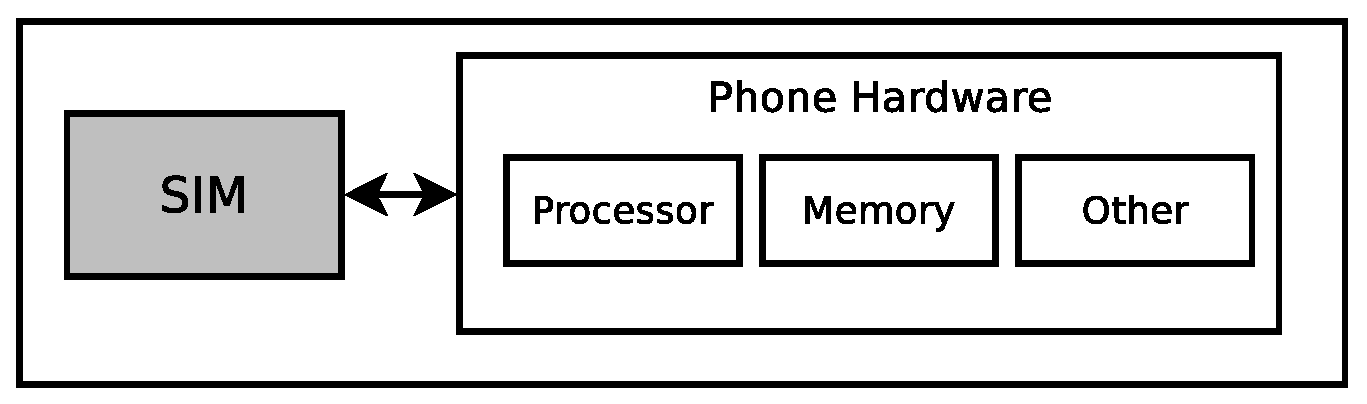
\includegraphics[width=0.9\textwidth]{images/SIM_in_GSM}
\caption[UICC running SIM application in GSM]
{
A UICC (SIM) card as used in GSM holds the Mobile Network Operator's secret key.
}
\label{fig:gsm_sim}
\end{figure}

These types of cards, also known as SIM cards, remain property of the \textit{Mobile Network Operator} (MNO) after distribution, much like a bank card or passport remain the property of their respective issuers. %TODO referentie
The contents of the card may normally not be modified by third parties.
Due to this, the current generation of mobile devices lacks a common infrastructure for third parties to make use of such a secure computation platform for their own applications.

%These third parties need to be elevated to the role of \textit{Trusted Service Manger}
%MARK: In de tekst hieronder moet duidelijk worden, dat NFC eist/vraagt dat een UICC wordt opgedeeld voor verschillende applicaties

% ERIK: SIM is een voorbeeld van een "Secure Element". Een Secure Element kan ook een andere smartcard chip in de telefoon zijn.

% In de telefoons die 'we' hebben is de SE geen onderdeel van de SIM, maar een los (al dan niet trusted) component.
%MARK: zullen we dit verder uitbreiden in het architectuur hoofdstuk en dit hier niet noemen?


%ERIK Waarom is de architectuur van GSM zoals-ie is & hoe breidt NFC dat uit? Er zijn tig opties van NFC telefoons, dus we kunnen niet overal diep op ingaan.

\subsection{Secure elements}
%Modern RFID cards can have features similar to smart cards, which means that NFC devices aiming to be truly compatible with RFID applications must also allow for similar functionality.
Just like SIM cards and RFID cards, NFC-enabled handsets require a secure storage and processing module to be included in their design as conventional storage on and operation of mobile devices are liable to tampering by the user or malicious third party.
%NFC, being grounded in RFID technology, provides some security capabilities previously unavailable in mobile devices.
%These capabilities require storage of sensitive data and code, for which a \textit{Secure element} is needed.
%Currently, four different configurations for a secure element are possible, of which the integration on a regular UICC/SIM is suggested as the most likely candidate to be used.
Secure storage for NFC applications similar to that provided by smart cards has been implemented in the \textit{Secure Element} (SE) architecture.
The software on the SEs can be updated over-the-air by a \textit{Trusted Services Manager} (TSM), provided the TSM's certificate is trusted by it.
Several possible configurations proposed by \textit{GlobalPlatform}, the industry forum for smart card infrastructure development, are outlined below. \cite{Reveilhac:2009:PSE:1548884.1549404,GlobalPlatformSEs}

%The secure element to be used is a \textit{Universal Integrated Circuit Card} (UICC).
%This is a smartcard which is used in a mobile phone to connect to the GSM and UTMS network. % UICC toevoegen aan glossary, Uitleggen dat het SIM is
%Making use of a UICC is preferred because it has been deployed in real applications where it has proven to be reliable.
%It is re-usable and standardized, which means a user can switch handsets easily, their personalized secure. 


%\textbf{TODO}
%A good reference on the feasibility of secure data and code in mobile devices is given in \cite{Reveilhac:2009:PSE:1548884.1549404}.
%Explain that the technical workings of these different devices are equivalent, but different configurations belong in different trust models.


%ERIK: figuren toevoegen van verschillende telefoon architecturen. 

% SIM ---> telefoon		SIM = secure, tamper-resitent, authenticatie van telefoon aan het netwerk	marketing redenen (onderscheid welke onderdelen van wie zijn) SIM is van de telco
% a SIM ---> telefoon ---> SE 	SmartMX contactless smartcard  (nokia)
% b SD kaart als a maar vervangbaar SE
% c NFC-SIM

%The problem of a malicious user can be mitigated by making use of a \textit{Secure Element} (SE) for storing sensitive information.
%Because of its sheer microscopic scale, it is very difficult and costly for an attacker to tamper with the function of this device.

%Below we will discuss a number of different ways such a secure element can be implemented on a mobile device. 

%\subsubsection{Integrated Secure Element}
\begin{enumerate}

\begin{item}
One option would be to integrate the SE in the handset hardware directly.
This works for the intended cryptographic use, but limits the device to communicate with the services using its pre-programmed certificates, unless it is capable of securely updating itself with new certificates.

%Nokia has released a phone like this in 2006 (the Nokia 6131 NFC) . %with NFC as a feature.
%The architecture of this phone consists of a SIM card, antenna and an internal Secure Element.
%The same layout of this architecture can also be used in other mobile devices, see figure \ref{fig:integrated_se}.

The handset hardware consists of the usual components like a processor, memory and possibly others, but also the hardware to provide NFC features and an embedded secure element.
The downside to this design is that the data contained in the SE is not easily portable to a new NFC device.
%The secure element stores sensitive data and enables tag and smart card emulation.
%In the case of the Nokia phone it is divided in two subcomponents, a Java Card, used for payment, and Mifare 4k, used for ticketing.

\begin{figure}
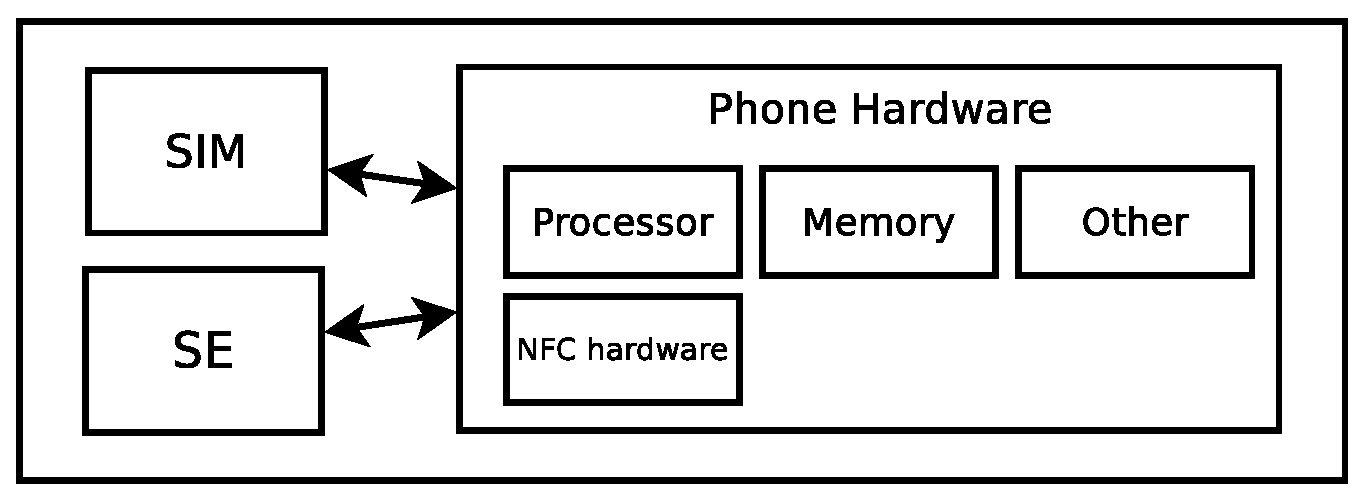
\includegraphics[width=0.9\textwidth]{images/phone_with_SE_nokia}
\caption[Handset with embedded Secure Element]
{
An embedded secure element
}
\label{fig:integrated_se}
\end{figure}
\end{item}

%security problems for this architecture:

%\subsubsection{Modular Secure Element}
\begin{item}
Another option is a flash memory card like a \textit{Secure Digital} (SD) card which houses all the hardware needed to enable NFC and also the secure element, as depicted in figure \ref{fig:modular_se}.
%( http://www.nearfieldcommunicationsworld.com/2009/01/12/3485/tyfone-puts-nfc-into-microsd-cards/)
In this configuration a third party can issue an SD card to its customers which provides NFC functionality without relying on any aspect of the handset to handle confidential data. If the user wishes to use applications from several third parties, they need to SD cards from all of those parties. This can be a downside, because the user has to switch the SD card if they want to use a different application.
\begin{figure}
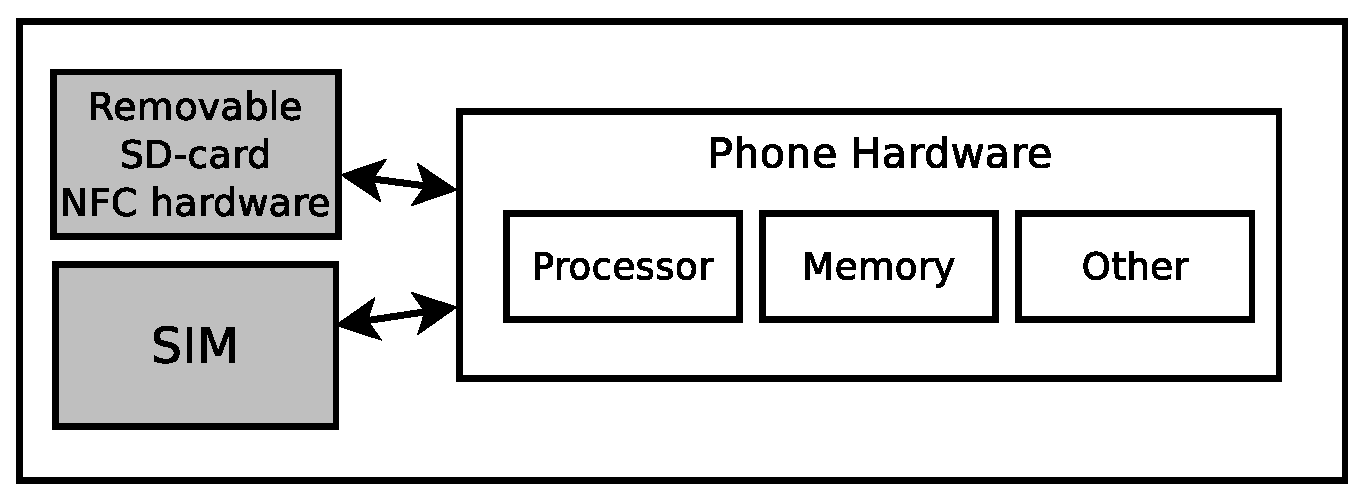
\includegraphics[width=0.9\textwidth]{images/SD_NFC}
\caption[SE in SD package]
{
A secure element in an SD package
}
\label{fig:modular_se}
\end{figure}
\end{item}

%security problems for this architecture: SD card might get stolen and used by somebody else.
%\subsubsection{Multiple SIM cards}
\begin{item}
Related to the above architecture is the one depicted in figure \ref{fig:multi_sim}.
Here the architecture consists of a handset with multiple UICC slots.
In this design various applications have access to their own UICC which takes on the role of an SE.
This way, applications from different providers can coexist on the handset, without the need for them to trust one another or a TSM operating on their behalf. % there is no problem with splitting the resources of one SIM card and the trust issue between different companies.
\begin{figure}
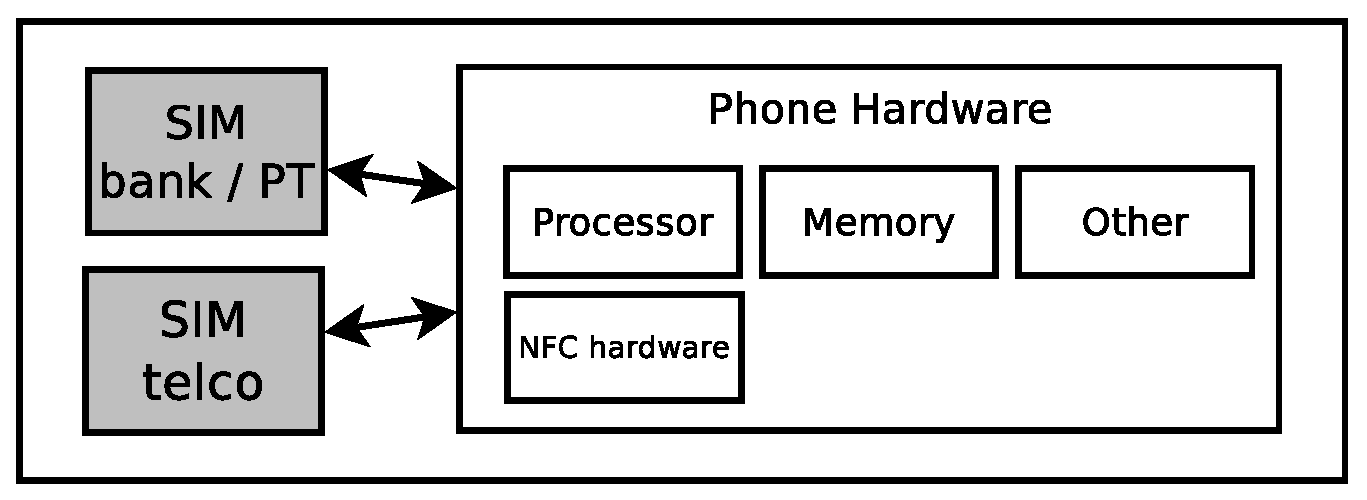
\includegraphics[width=0.9\textwidth]{images/meerdere_sims}
\caption[Multiple SIM cards]
{
Multiple SIM cards for different applications
}
\label{fig:multi_sim}
\end{figure}
\end{item}

\begin{item}
%\subsubsection{Trusted SIM card}
It is also possible to split the resources available on the SE between various parties, granted they trust each other to not abuse the privilege of being able to access one another's data.
This sharing of resources is possible because smart cards in general are becoming more powerful.
This makes two different architectures possible.
The first one, as pictured in figure \ref{fig:sim_se}, uses the SIM card as secure element.
In this design, the handset will include the NFC communication hardware and utilize a UICC (SIM card) with applications from the Mobile Network Operator and applications from various third parties chosen by the user, e.g. a bank for payment and a public transport company. 
The second option resembles a combination of the first one and the one with the SD card architecture.
Here a SIM card has all the hardware needed to make NFC possible and it also acts as a secure element (see figure \ref{fig:integrated_se}).
Like the first option, the resources of the SIM card will be split among the involved parties.
\begin{figure}
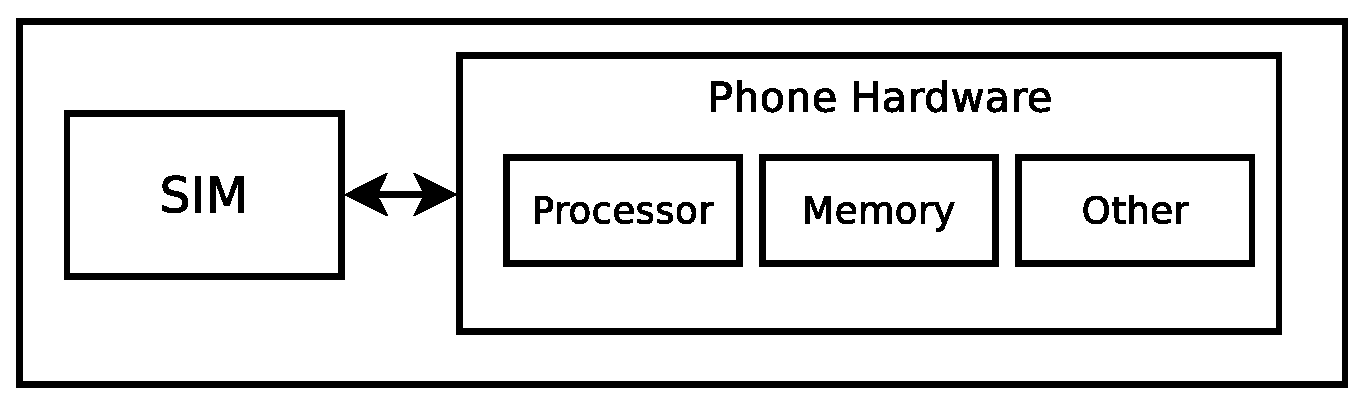
\includegraphics[width=0.9\textwidth]{images/SIM_is_SE}
\caption[Trusted SIM cards]
{
Trusted SIM card running multiple applications
}
\label{fig:sim_se}
\end{figure}
\end{item}

\end{enumerate}

%hier moet nog een bron voor gevonden worden
%security problems for this architecture: SIM card might get stolen and used by somebody else
%hier moet nog een bron voor gevonden worden
%security problems for this architecture: SIM card might get stolen and used by somebody else


%\textbf{TODO} A good reference for cyclic dependency of stakeholders can be found in the GlobalPlatform technical report.


% TODO hoort bij Wireless communication, terwijl 3.2 (Secure Elements) heel ergens anders over gaat
%\subsection{Standardization}
%NFC has been described by NFCIP-1 (Near Field Communication Interface Protocol 1) first on ISO18092, ECMA340 and ETSI %TS102 and also NFCIP-2 defined in ISO 21481, ECMA352 and ETSI TS102 312.
%With NFCIP-2, NFC became compliant with the RFID standards of ISO14443 and ISO15693.


% diagram van NFC communicatie

%TODO RFiD card vs NFC - verschil vd terminal
%                      - live GSM verbinding met de bank
%TODO Online vs Offline
%                      - privacy gevoeligheid

%\section{Wireless communication}
%The distance at which the NFC communication takes place is 10 cm, operates at the 13.56 MHz frequency and it has a transfer speed of 106, 216, 424 kbit/s.
%promising secure element alternatives for NFC technology. */


%\subsection{Advantages and Limitations}
%\textbf{TODO}

% Toetsenbord en display feature (semi-trusted terminal, moeilijker te tamperen)

% Voorbeeld telefoon met gewone sim en NFC SD card adapter
% Bankier kan heir apps op installeren

% Voorbeeld telefoon met meerdere sims

% Vorobeeld SIM en losse SE, met trusted code

% Voorbeeld SIM van KPN, met apps van de bank

%TODO Uitzoeken:
% Rabomobiel - SIM vd rabobank


